\documentclass[12pt]{article}

% Language setting
% Replace `english' with e.g. `spanish' to change the document language
\usepackage[english]{babel}

% Set page size and margins
% Replace `letterpaper' with `a4paper' for UK/EU standard size
\usepackage[a4paper,top=2cm,bottom=2cm,left=2cm,right=2cm,marginparwidth=1.75cm]{geometry}

% Useful packages
\usepackage{amsmath}
\usepackage{graphicx}
\usepackage[colorlinks=true, allcolors=blue]{hyperref}
\usepackage{tcolorbox}
\usepackage[utf8]{inputenc}
\usepackage{bm}

\linespread{1.25}
\setlength{\parindent}{0px}

\title{Lecture 03}
\author{Random Variables, Probability and Likelihood}

\begin{document}
\maketitle{}

\section{Generalization and Overfitting}
Fitting a model perfectly to the training data leads to poor predictions as there will almost be noise present.
\vspace{1.5em}

There is a common trade-off between generalization and overfitting. We would prefer to generalize our model instead of overfitting it so that it can be practical. 
\vspace{1.5em}

Here is how a generalized and overfitted model looks like (the data points used are not the best to show an overfitted model..):
\vspace{1.5em}

\begin{figure}[h]
\centering

\begin{minipage}[b]{0.4\linewidth}
  \centering
  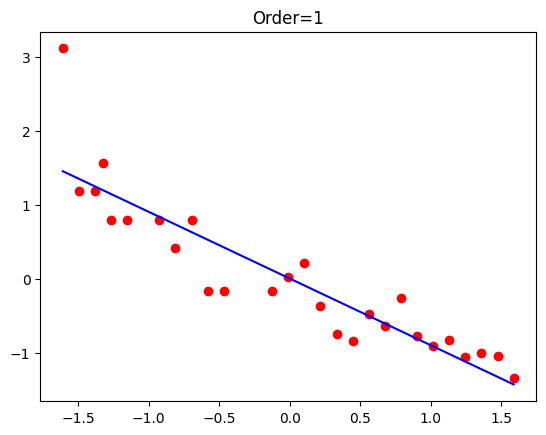
\includegraphics[width=\linewidth]{images/lecture_03/img_1.png}
  \caption{Generalized model}
  \label{fig:img_1}
\end{minipage}
\hspace{0.03\linewidth}
\begin{minipage}[b]{0.4\linewidth}
  \centering
  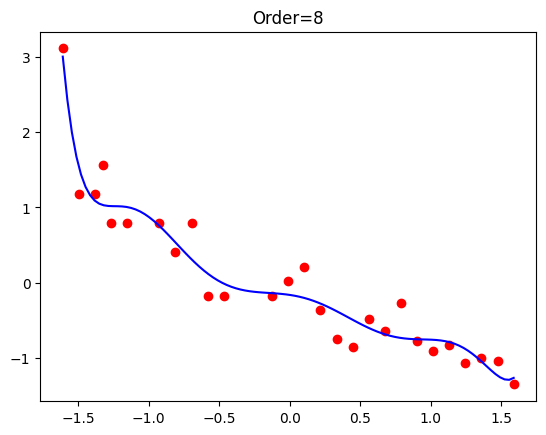
\includegraphics[width=\linewidth]{images/lecture_03/img_2.png}
  \caption{Overfitted model}
  \label{fig:img_2}
\end{minipage}

\end{figure}

\newpage
\section{Modelling Errors}

Errors exist in all models, and we should not ignore them. Instead, we can use them as an indication of how confident are the model predictions. That is, how certain we feel about the predicted values.
\vspace{1.5em}

\begin{figure}[h]
\centering

\begin{minipage}[b]{0.4\linewidth}
  \centering
  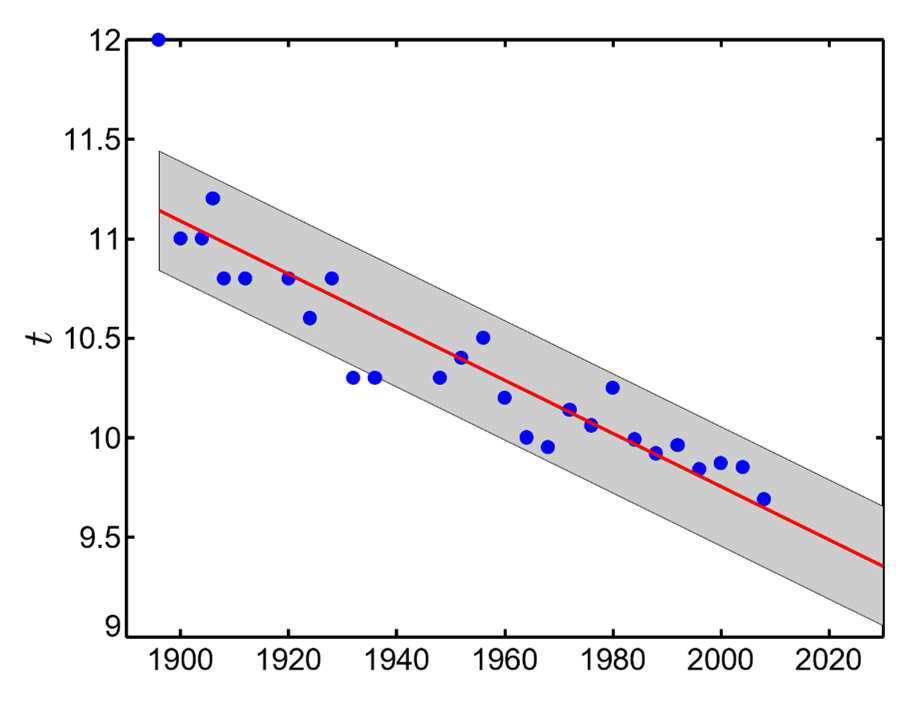
\includegraphics[width=\linewidth]{images/lecture_03/img_3.png}
  \label{fig:img_3}
\end{minipage}
\hspace{0.03\linewidth}
\begin{minipage}[b]{0.4\linewidth}
  \centering
  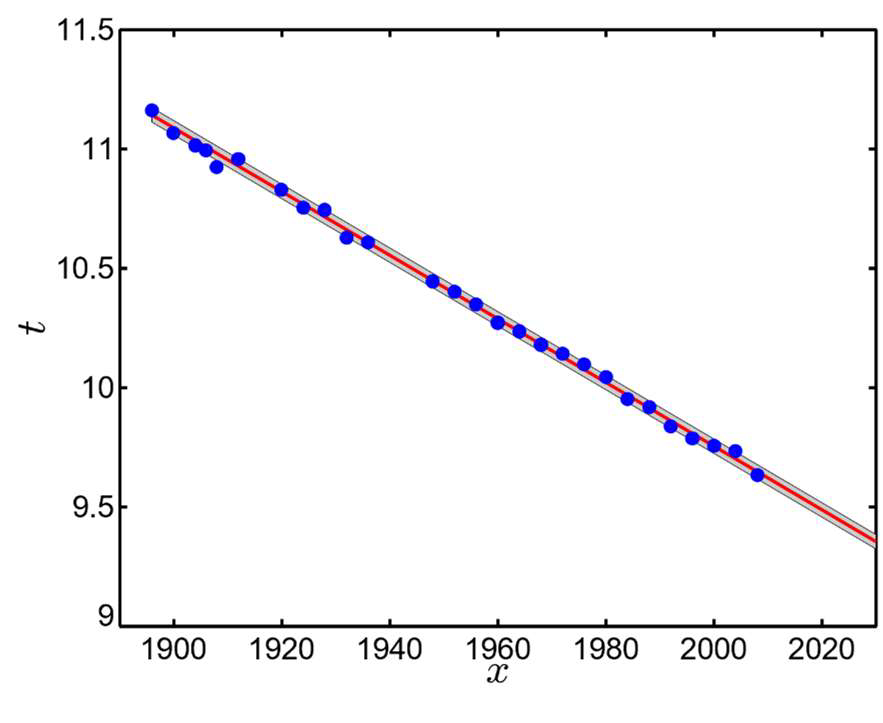
\includegraphics[width=\linewidth]{images/lecture_03/img_4.png}
  \label{fig:img_4}
\end{minipage}

\end{figure}

The narrower the shaded region, the more \textbf{precise} the model predictions are, \textbf{but not necessarily accurate}.

\subsection{Additive Errors}
We can include noise in our training models by adding an additive term:
\vspace{0.5em}

\[
t_n = \mathbf{w}^\top \mathbf{x}_n + \epsilon_n
\]
\vspace{0.5em}

Since noise is random, we can model it as a random variable. We can model noise in a Gaussian (normal) distribution as below:
\vspace{0.5em}

\[
p(\epsilon \mid \mu, \sigma^2) = \frac{1}{\sigma \sqrt{2\pi}} \exp\left\{ -\frac{1}{2\sigma^2} (\epsilon - \mu)^2 \right\}
\]
\vspace{0.5em}

By modelling noise using the Gaussian distribution, we are able to quantify uncertainty, generate synthetic data and use probabilistic interpretations like confidence intervals and \textbf{likelihood}. 


(On a side note, modelling noise using Gaussian, the output becomes a random variable too.)

\newpage
\section{Likelihood}
The likelihood value is a measure of how likely an observed outcome under a model, or evaluates how well a model explains an observed outcome. Likelihood is also the value of the \textbf{probability density function} evaluated from a given dataset and a fixed model (weight parameters, mean and variance values are fixed).
\vspace{0.5em}

\[
\text{Likelihood} = p(t \mid \mathbf{x}_n, \mathbf{w}, \sigma^2) = \mathcal{N}(\mathbf{w}^\top \mathbf{x}_n, \sigma^2)
\]
\vspace{0.5em}

We can use likelihood to evaluate model quality across different models. The model with higher total likelihood (log-likelihood) across all data is better.

\subsection{Simple Analog}
To further solidify our understanding of likelihood, imagine a weather model predicts:

\begin{quote}
\centering{“Tomorrow’s temperature should be around 25\textdegree C with ±1\textdegree C variance”}
\end{quote}

But then, it turns out to be \textbf{35\textdegree C}. 
\vspace{1.0em}

\begin{tcolorbox}[colback=blue!10, colframe=blue!80!black, sharp corners, boxrule=0.4pt]
  The \textbf{likelihood} of 35\textdegree C under that model is \textbf{very low}, which means that this model is not good at explaining this event. Maybe the model needs an update, by changing the mean and variance values, or even the weight parameters.
\end{tcolorbox}

\subsection{Likelihood Optimization}
The mean, variance and weight parameters that maximizes the likelihood value (under Gaussian noise assumption) will also minimize the squared error of a linear regression model. It is the \textbf{maximum likelihood estimation}.
\vspace{1.5em}

To compute the optimum weight ($\hat{\bm{w}}$), we can use this equation:
\[
\hat{\bm{w}} = (\mathbf{X}^\top \mathbf{X})^{-1} \mathbf{X}^\top \mathbf{t}
\]

And we use this equation to compute the optimum variance ($\hat{\sigma}^2$):
\[
\hat{\sigma}^2 = \frac{1}{N} (\mathbf{t} - \mathbf{X} \hat{\bm{w}})^\top (\mathbf{t} - \mathbf{X} \hat{\bm{w}})
\]

\end{document}